\documentclass[12pt]{article}
\usepackage{graphicx}
\usepackage{amsmath}

\begin{document}
CSCI-4100 Assignment 9\\
Yichuan Wang \\
RIN:661414395\\\\
1. 8th order Legendre transform gives 45 features. There are 300 samples. The dimension of Z is therefore $300\times45$\\\\
2. Overfitting\\
The decision boundary is shown both training data and test data. \\
On training data: $E_{cv}=0.0810=$ $E_{test}=0.01723$\\
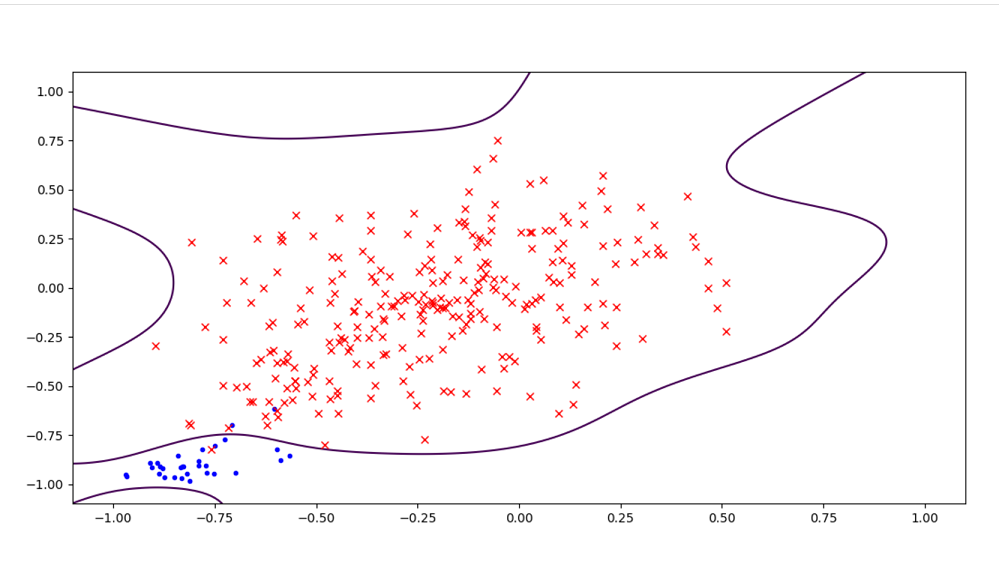
\includegraphics[scale=0.5]{images/lambda_0_train}\\
Same decision boundary on test data:\\
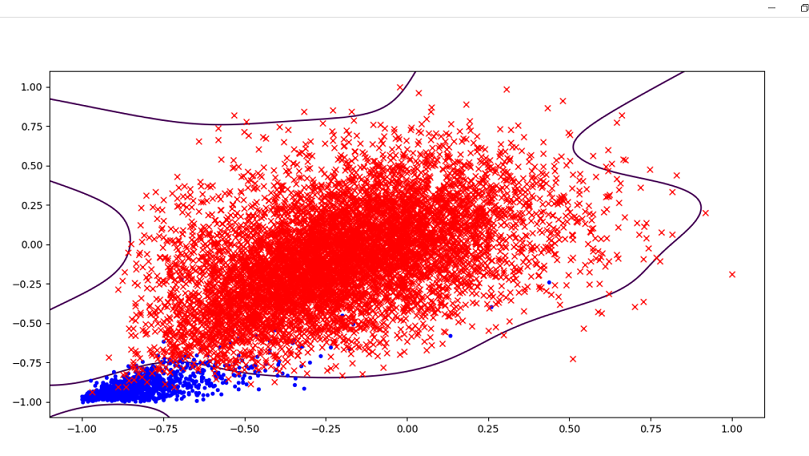
\includegraphics[scale=1]{images/lambda_0_test}\\
As shown in the images, the decision boundary omitted the outer region of red points, and that is overfitting. \\\\
3. Regularization\\
The decision boundary is shown both training data and test data. \\
On training data: $E_{cv}=0.05045$ $E_{test}=0.01489$\\
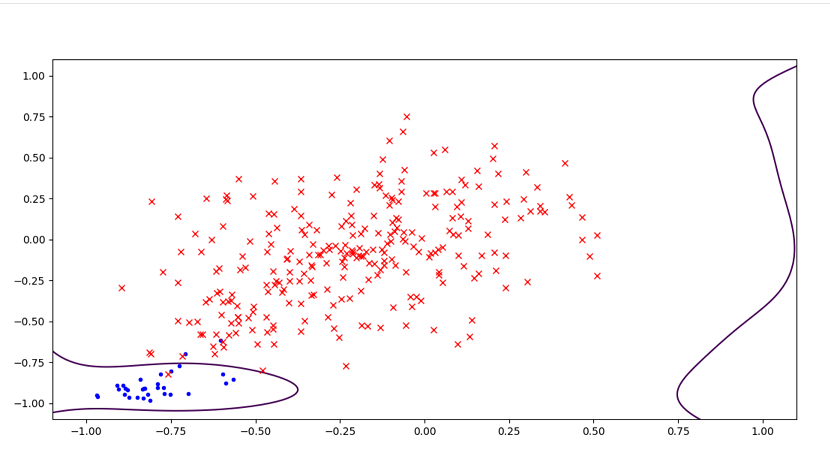
\includegraphics[scale=0.5]{images/lambda_2_train}\\
Same decision boundary on test data:\\
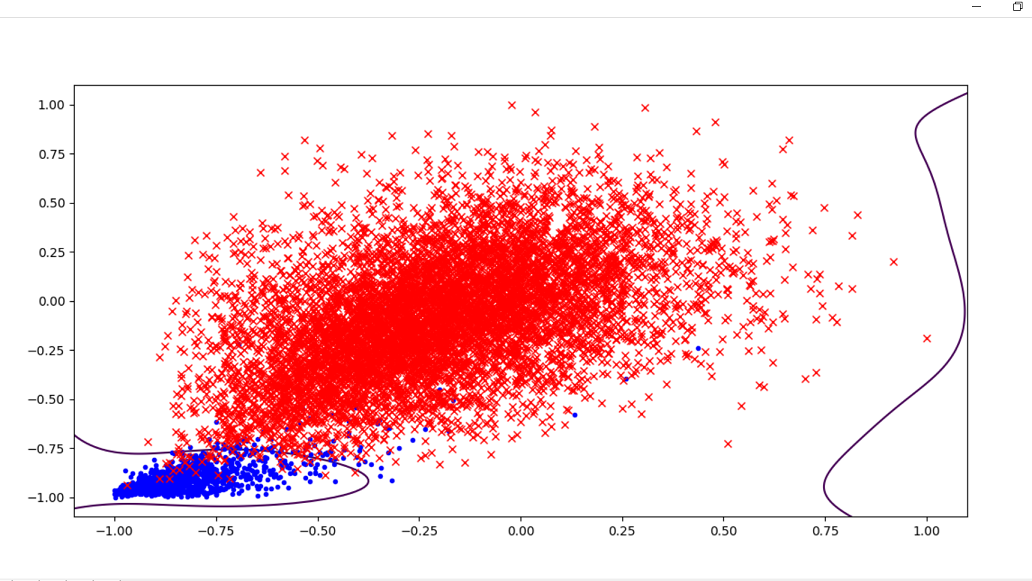
\includegraphics[scale=0.5]{images/lambda_2_test}\\
A clear boundary is shown on test data between +1 data points and -1 data points. There is no overfitting or underfitting. \\\\
4. Cross Validation\\
The red curve is $E_{cv}$, and the blue curve is $E_{test}$\\
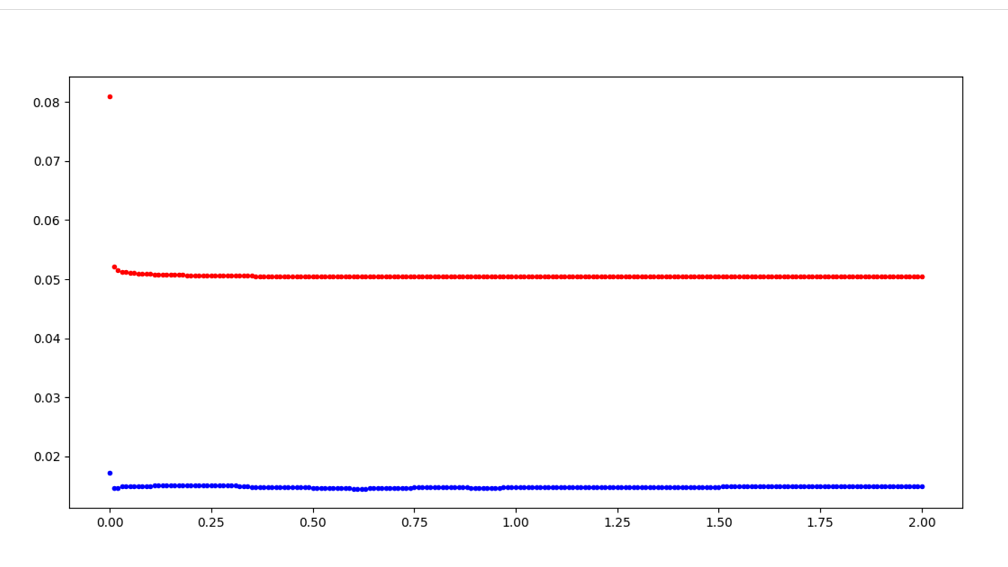
\includegraphics[scale=0.5]{images/ecv_vs_etest}\\
At $\lambda=0$, $E_{cv}$ is very large($E_{cv}=0.081$). As regularization increases, $E_{cv}$ quickly converges to a smaller value. Same behavior pattern applies to $E_{test}$: Relatively large at no regularization ($E_{test}=0.017$), then quickly converges to a smaller value ($E_{cv}=0.015$). The change in $E_{test}$ is smaller than that of $E_{test}$. The stable value of $E_{cv}$ is around 3 times higher than that of $E_{test}$.\\\\
5. Pick $\lambda^*$
The regularization that gives best $E_{cv}$ is $\lambda=1.17$, where $E_{cv}=0.05039$\\
Decision boundary:\\
Training data:\\
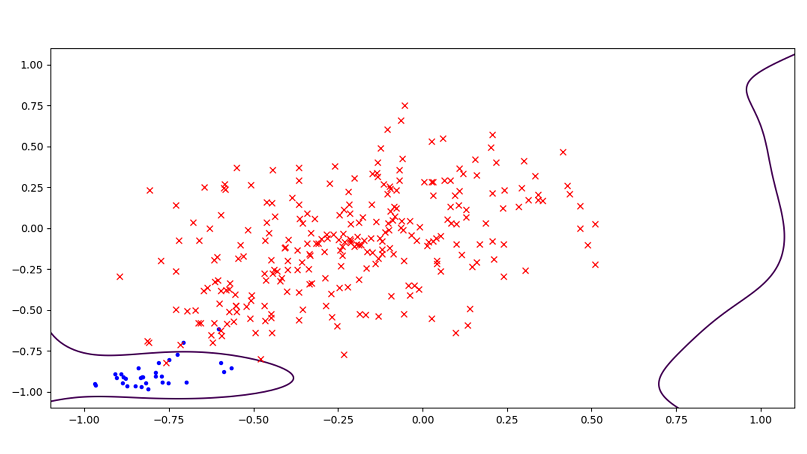
\includegraphics[scale=0.5]{images/lambda_star_train}\\
Testing data:\\
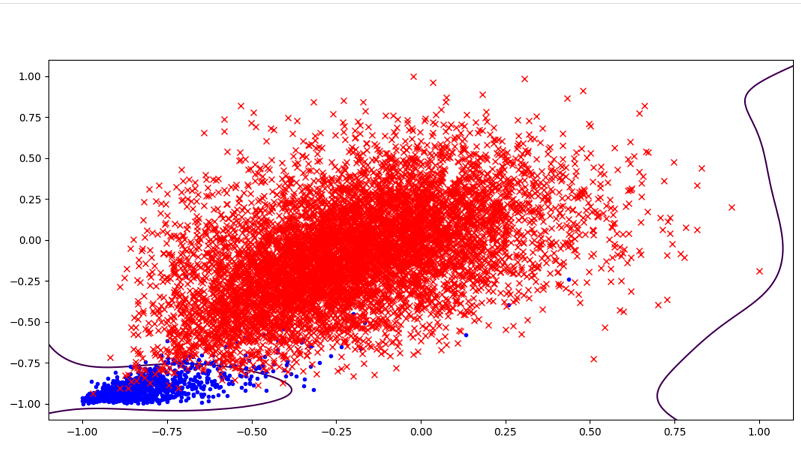
\includegraphics[scale=0.5]{images/lambda_star_test}\\

6. At $\lambda=1.17$, we have $E_{test}=0.01478$. The testing data contains $9298-300=8998$ data points. $E_{out}$ can be calculated as following ($\delta=0.05$):
$$E_{out}<E_{test}+\sqrt{\frac{1}{8998\times 2}ln\frac{2\times 1}{0.05}}=0.01478+0.01432=0.0291$$\\
7. No, $E_{cv}(\lambda^*)$ is unbiased. For each leave-one-out validation, the test data point does not involve in the training, so every test in the validation cycle is an unbiased estimate of $E_{out}$\\\\
8. Yes, there is data snooping. We normalized data before we separate it into training group and testing group. In this case, the value of shift and scale contains information from the testing data, and this information is distributed to all the data points, from which we selected 300 points for training. To fix this, we need to separate the data first, and normalize only the training data. We use the scale and shift obtained from training data to normalize our test data.  
\end{document}












